
\documentclass[12pt]{article}

\usepackage{multicol}
\usepackage[a4paper, portrait, margin=1in]{geometry}
\usepackage{graphicx}
\graphicspath{{images/}}
\usepackage{array}
\usepackage{hyperref}

\hypersetup{pdfborder={0 0 0}}

\usepackage{etoolbox}
\patchcmd{\abstract}{\null\vfil}{}{}{}



\title{Auto-Tagging Selection Test}
\date{2015-07-03}
\author{Shubham Gupta}

\begin{document}

	% Title Page
	\begin{titlepage}
		\begin{center}
			\vspace*{20mm}
			\LARGE
			\textbf{eYSIP-2015}\\
			\vspace{15mm}
			\Huge\textsc{Auto-Tagging Online Selection Test}\\
			\vfill
			\Large
			\textbf{Intern}\\
			Shubham Gupta\\
			suvam8694@gmail.com\\
			+91 83 760 27800\\
			\vspace{10mm}
			\textbf{Project Mentor}\\
			Mr. Amiraj Dhawan\\
			amirajdhawan@gmail.com\\
			+91 99 206 78775\\
			\vspace{10mm}
			\textbf{Duration}\\
			05/06/2015 to 17/07/2015
			\vspace{20mm}
		\end{center}
	\end{titlepage}
	
	
	\tableofcontents
	
	
	% Start the report
	
	% Abstract of Report
	\newpage
	\begin{abstract}
		While Moore's Law makes machines faster, Machine Learning
		makes them smarter. Machine Learning is an active research
		area which has been successfully applied for solving a lot of
		challenging problems having practical significance. Here we
		have applied machine learning to solve such a problem. The task
		was to automatically assign a difficulty level to each question
		in the eYRC-2015 Online Selection Test based on the data about
		performance of students. For solving this problem we experimented
		with different machine learning algorithms for example k-Means
		Clustering, Expectation Maximization Algorithm etc.\newline
		The results obtained here have practical significance for many
		reasons. As an example, using the results obtained here, questions
		can be combined to form balanced sets, all of which have similar
		difficulty level, to ensure a higher level of fairness in a future
		iteration of the test.
	\end{abstract}
	
	
	% Begin the Actual Content
	\newpage
	
	
	% Write the Problem Statement in Objective
	\section{Objectives}
	eYantra conducts an online test to select student teams for eYRC. 
	The questions used for eYRC-2015 are manually assigned
	a difficulty level prior to the commencement of the test based on
	experience of question maker. Since there are a lot of questions
	and many different question makers, the manually assigned difficulty
	levels are not reliable due to the \textit{relative nature} of
	difficulty of questions.\newline
	There are two main objectives:
	
	\subsection{Auto-Tagging}
	Using the data generated during eYRC-2015 Online Selection Test, the
	task is to determine the accuracy of manually assigned difficulty
	levels and also suggest corrections to them based on performance
	of students. 
	
	\subsection{Performance Prediction}
	This task involves finding correlations between various aspects in the
	profile of a student and performance of the student and hence use the
	deduced machine learning model to predict the performance of a student
	in the future iteration of the test given his/her profile.\newline	
	
	
	% Write the Completion Status
	\section{Completion Status}
	Part 1 i.e. \textbf{Auto-Tagging} has been completed while the work 
	on part 2 i.e. \textbf{Performance Prediction} is in progress. Hence
	this report focuses on Part 1 only.
	
	
	% Write Results and Discussions
	\section{Results and Discussions}
	A variety of different machine learning algorithms were applied to 
	solve the \textit{Auto-Tagging} problem. Many combinations of features
	and algorithms were considered. Some of the main ones have been described
	here:
	
	% Describe Neural Network
	\subsection{Neural Network}
	Both complete and sparse neural networks were implemented. This was
	the first approach that was used. Here the problem was viewed as a 
	supervised learning problem where the assumption was that majority of
	the manually assigned tags are correct. Under this assumption it was
	predicted that the network will generalize well and automatically rectify
	the incorrect tags which are present in minority.
	It was discovered later that this assumption was wrong. This approach
	was tried with different combinations of features but the results were
	unsatisfactory. 
	
	\paragraph{Estimated Manual Tagging Accuracy: 52.45\%}
	
	
	% Describe k-Means Clustering
	\subsection{k-Means Clustering}
	k-Means Clustering is an unsupervised learning algorithm used for
	clustering the data into semantically sound clusters. This algorithm
	was used with many different combination of features. The most satisfactory
	output was obtained by using the following three features:
	\begin{enumerate}
	\item Fraction of people who solved a question correctly.
	\item Fraction of people in top five percentile who solved the question
	correctly.
	\item Average marks of people who did not attempt the given question or
	solved it incorrectly.
	\end{enumerate}
	
	This output has been shown below:
	\begin{figure}[h]
	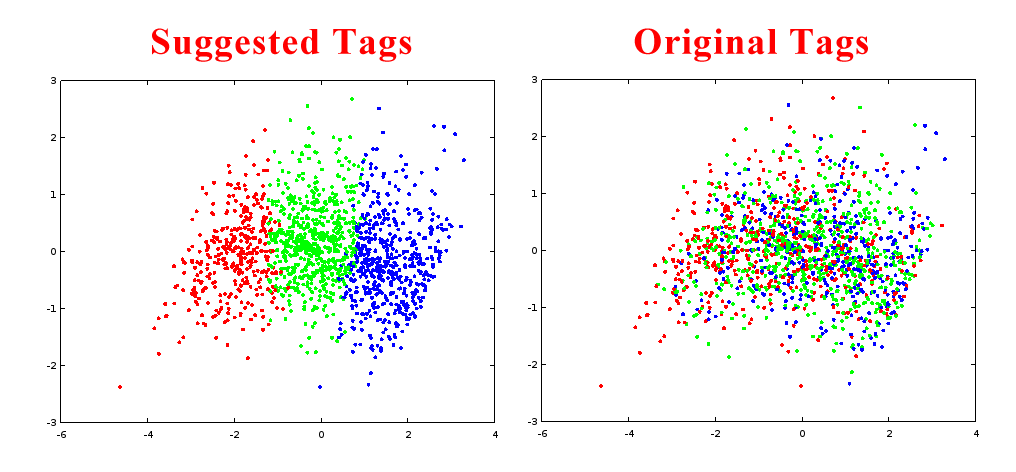
\includegraphics[width=\textwidth]{ClusteringOutput}
	\end{figure}
	
	\begin{center}
	\begin{table}[h]
		\begin{tabular}{ | m{2cm} | m{1.7cm} | m{1.3cm} | m{1.3cm} | m{1.5cm} | m{1.3cm} | m{1.3cm} | m{1.3cm} | }
		\hline
		\textbf{Feature} & \textbf{Level} & \textbf{Min} & \textbf{Q1} & \textbf{Median} & \textbf{Q3} & \textbf{Max} & \textbf{Mean}\\ 
		\hline
		\textbf{Feature 1} & \textbf{Easy Medium Hard} & -0.515 \hspace{5mm}-1.359 \hspace{5mm}-1.686 & 0.842 \hspace{5mm}-0.470 \hspace{5mm}-1.213 & 1.370  \hspace{5mm}-0.106 \hspace{5mm}-0.946 & 1.818 \hspace{5mm}0.373 \hspace{5mm}-0.605 & 2.934 \hspace{5mm}1.813 \hspace{5mm}1.106 & 1.318 \hspace{5mm}-0.031 \hspace{5mm}-0.860\\
		\hline
		\textbf{Feature 2} & \textbf{Easy Medium Hard} & -0.342 \hspace{5mm}-0.842 \hspace{5mm}-1.843 & 0.962 \hspace{5mm}-0.018 \hspace{5mm}-1.843 & 1.159  \hspace{5mm}0.409 \hspace{5mm}-1.092 & 1.159 \hspace{5mm}0.730 \hspace{5mm}-0.642 & 1.159 \hspace{5mm}1.159 \hspace{5mm}0.159 & 1.018 \hspace{5mm}0.377 \hspace{5mm}-1.139\\
		\hline
		\textbf{Feature 3} & \textbf{Easy Medium Hard} & -4.498 \hspace{5mm}-1.667 \hspace{5mm}-2.050 & -1.631 \hspace{5mm}-0.339 \hspace{5mm}0.159 & -1.091  \hspace{5mm}0.028 \hspace{5mm}0.589 & -0.623 \hspace{5mm}0.479 \hspace{5mm}1.132 & 1.104 \hspace{5mm}2.620 \hspace{5mm}3.380 & -1.134 \hspace{5mm}0.093 \hspace{5mm}0.662\\
		\hline
		\end{tabular}
		\caption{Statistics for k-Means Output}
	\end{table}
	\end{center}
	
	\paragraph{Estimated Manual Tagging Accuracy: 43.73\%}
	
	
	% Describe Competitive Learning
	\newpage
	\subsection{Competitive Learning}
	Competitive Learning is another unsupervised learning algorithm which can
	be used for	clustering of data. This algorithm can be implemented as
	a neural network. Autoencoder was used to encode features to feed input
	to the algorithm. Following two features were fed to autoencoder:
	\begin{enumerate}
	\item Fraction of people who solved a question correctly.
	\item Fraction of people in top five percentile who solved the question
	correctly.
	\end{enumerate}
	
	Best results were obtained when only these two features were used, 
	although other feature combinations were also tried. This algorithm
	is also faster than k-Means	clustering. Output has been shown below:
	\begin{figure}[h]
	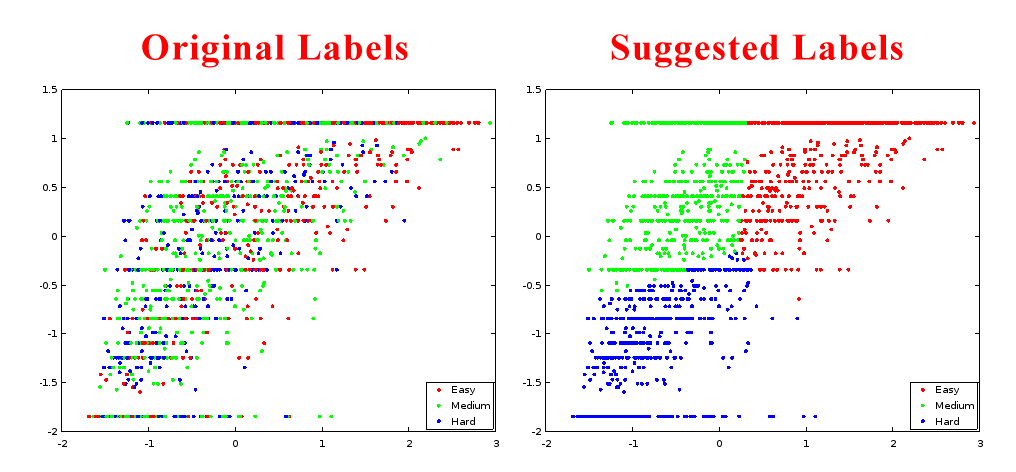
\includegraphics[width=\textwidth]{CompetitiveOutput}
	\end{figure}
	
	\begin{center}
	\begin{table}[h]
		\begin{tabular}{ | m{2cm} | m{1.7cm} | m{1.3cm} | m{1.3cm} | m{1.5cm} | m{1.3cm} | m{1.3cm} | m{1.3cm} | }
		\hline
		\textbf{Feature} & \textbf{Level} & \textbf{Min} & \textbf{Q1} & \textbf{Median} & \textbf{Q3} & \textbf{Max} & \textbf{Mean}\\ 
		\hline
		\textbf{Feature 1} & \textbf{Easy Medium Hard} & 0.234 \hspace{5mm}-1.503 \hspace{5mm}-1.686 & 0.652 \hspace{5mm}-0.695 \hspace{5mm}-1.211 & 1.051  \hspace{5mm}-0.419 \hspace{5mm}-0.886 & 1.580 \hspace{5mm}-0.096 \hspace{5mm}-0.414 & 2.934 \hspace{5mm}0.324 \hspace{5mm}1.106 & 1.169 \hspace{5mm}-0.412 \hspace{5mm}-0.781\\
		\hline
		\textbf{Feature 2} & \textbf{Easy Medium Hard} & -0.642 \hspace{5mm}-0.556 \hspace{5mm}-1.843 & 0.492 \hspace{5mm}-0.042 \hspace{5mm}-1.843 & 1.159  \hspace{5mm}0.409 \hspace{5mm}-1.092 & 1.159 \hspace{5mm}0.859 \hspace{5mm}-0.717 & 1.159 \hspace{5mm}1.159 \hspace{5mm}-0.175 & 0.804 \hspace{5mm}0.392 \hspace{5mm}-1.185\\
		\hline
		\end{tabular}
		\caption{Statistics for Competitive Learning Output}
	\end{table}
	\end{center}
	
	\paragraph{Estimated Manual Tagging Accuracy: 43.05\%}
	
	
	% Describe EM
	\newpage
	\subsection{Expectation Maximization Algorithm}
	Expectation Maximization algorithm can be used for \textit{soft clustering}.
	of the data. For this algorithm, a mixture of gaussians model was assumed.
	From the obtained soft clustering output, question labels were predicted
	by taking most likely tag for each question. The following features were used:
	\begin{enumerate}
	\item Fraction of people who solved a question correctly.
	\item Fraction of people in top five percentile who solved the question
	correctly.
	\end{enumerate}
	
	Best results were obtained when only these two features were used, 
	although other feature combinations were also tried. This algorithm provides
	a skewed output forcing many questions to fall in the medium difficulty
	level category. Output has been shown below:
	\begin{figure}[h]
	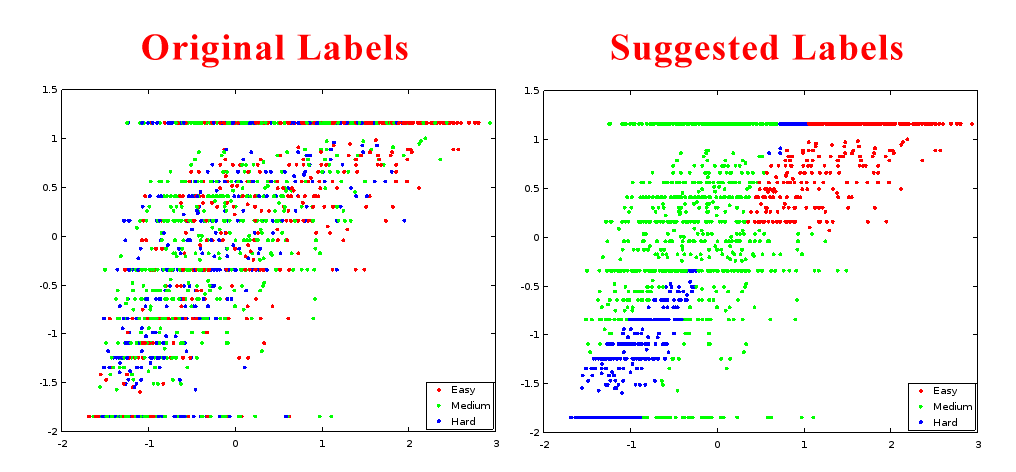
\includegraphics[width=\textwidth]{EMOutput}
	\end{figure}
	
	\begin{center}
	\begin{table}[h]
		\begin{tabular}{ | m{2cm} | m{1.7cm} | m{1.3cm} | m{1.3cm} | m{1.5cm} | m{1.3cm} | m{1.3cm} | m{1.3cm} | }
		\hline
		\textbf{Feature} & \textbf{Level} & \textbf{Min} & \textbf{Q1} & \textbf{Median} & \textbf{Q3} & \textbf{Max} & \textbf{Mean}\\ 
		\hline
		\textbf{Feature 1} & \textbf{Easy Medium Hard} & 0.355 \hspace{5mm}-1.519 \hspace{5mm}-1.686 & 0.986 \hspace{5mm}-0.671 \hspace{5mm}-1.250 & 1.412  \hspace{5mm}-0.265 \hspace{5mm}-0.979 & 1.824 \hspace{5mm}0.137 \hspace{5mm}-0.576 & 2.934 \hspace{5mm}1.485 \hspace{5mm}1.031 & 1.415 \hspace{5mm}-0.271 \hspace{5mm}-0.762\\
		\hline
		\textbf{Feature 2} & \textbf{Easy Medium Hard} & 0.068 \hspace{5mm}-1.843 \hspace{5mm}-1.843 & 0.559 \hspace{5mm}-0.342 \hspace{5mm}-1.843 & 0.971  \hspace{5mm}0.159 \hspace{5mm}-1.242 & 1.159 \hspace{5mm}0.659 \hspace{5mm}-0.717 & 1.159 \hspace{5mm}1.159 \hspace{5mm}1.159 & 0.846 \hspace{5mm}0.081 \hspace{5mm}-0.983\\
		\hline
		\end{tabular}
		\caption{Statistics for EM Output}
	\end{table}
	\end{center}
	
	\paragraph{Estimated Manual Tagging Accuracy: 45.40\%}
	
	
	% Describe Weighted Clustering
	\newpage
	\subsection{Weighted Clustering}
	The core idea behind using weighted clustering is to allow students
	who have got higher scores to contribute more towards clustering as
	compared to those students who have got lower scores. The rationale
	behind using such a strategy is that students with higher scores give
	more authentic data containing fewer random guesses. The following
	weighted features were used with k-Means Clustering to achieve weighted
	clustering:
	\begin{enumerate}
	\item Fraction of people who solved a question correctly adjusted by weight.
	\item Average weight adjusted marks of students who did not attempt a given 
	question or solved it incorrectly.
	\end{enumerate}
	
	Weighing of features is used by assigning higher weights to students who
	have got higher scores and vice versa. This in effect gives rise to a 
	weighted clustering algorithm without changing the core algorithm. One
	difficulty is estimating the accuracy of suggested tags since now we
	are no longer dealing with original features, hence result analysis has been
	done using original features from k-Means Clustering.
	\begin{figure}[h]
	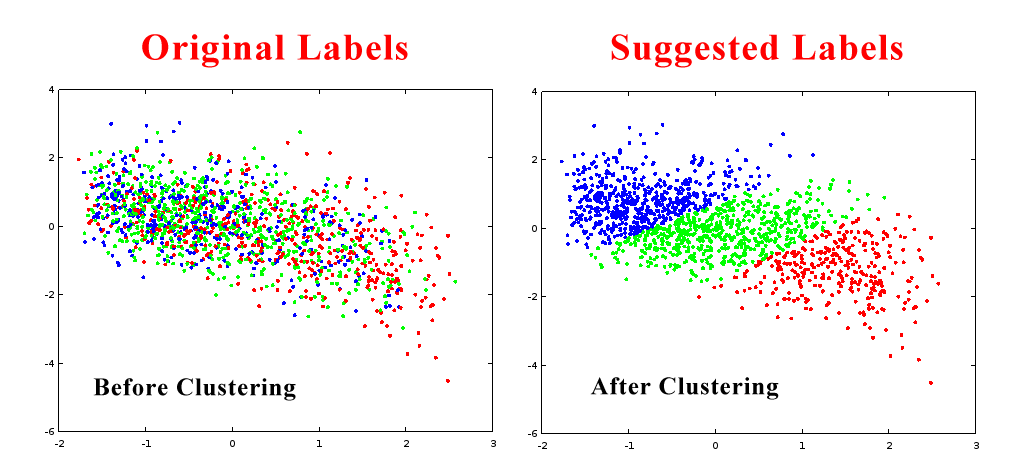
\includegraphics[width=\textwidth]{WeightedClusteringOutput}
	\end{figure}
	
	\begin{center}
	\begin{table}[h]
		\begin{tabular}{ | m{2cm} | m{1.7cm} | m{1.3cm} | m{1.3cm} | m{1.5cm} | m{1.3cm} | m{1.3cm} | m{1.3cm} | }
		\hline
		\textbf{Feature} & \textbf{Level} & \textbf{Min} & \textbf{Q1} & \textbf{Median} & \textbf{Q3} & \textbf{Max} & \textbf{Mean}\\ 
		\hline
		\textbf{Feature 1} & \textbf{Easy Medium Hard} & -0.515 \hspace{5mm}-1.504 \hspace{5mm}-1.686 & 0.907 \hspace{5mm}-0.447 \hspace{5mm}-1.188 & 1.424  \hspace{5mm}-0.013 \hspace{5mm}-0.883 & 1.851 \hspace{5mm}0.483 \hspace{5mm}-0.506 & 2.934 \hspace{5mm}2.165 \hspace{5mm}1.485 & 1.380 \hspace{5mm}0.040 \hspace{5mm}-0.802\\
		\hline
		\textbf{Feature 2} & \textbf{Easy Medium Hard} & -1.843 \hspace{5mm}-1.843 \hspace{5mm}-1.843 & 1.159 \hspace{5mm}-0.183 \hspace{5mm}-1.468 & 1.159  \hspace{5mm}0.409 \hspace{5mm}-0.842 & 1.159 \hspace{5mm}0.826 \hspace{5mm}-0.342 & 1.159 \hspace{5mm}1.159 \hspace{5mm}1.159 & 1.020 \hspace{5mm}0.238 \hspace{5mm}-0.818\\
		\hline
		\textbf{Feature 3} & \textbf{Easy Medium Hard} & -4.498 \hspace{5mm}-1.850 \hspace{5mm}-1.121 & -1.733 \hspace{5mm}-0.494 \hspace{5mm}0.379 & -1.127  \hspace{5mm}0.136 \hspace{5mm}0.741 & -0.731 \hspace{5mm}0.198 \hspace{5mm}1.238 & 0.481 \hspace{5mm}1.979 \hspace{5mm}3.380 & -1.227 \hspace{5mm}-0.137 \hspace{5mm}0.822\\
		\hline
		\end{tabular}
		\caption{Statistics for EM Output (Using Features from k-Means Clustering)}
	\end{table}
	\end{center}
	
	\paragraph{Estimated Manual Tagging Accuracy: 43.18\%}
	
	
	% Discuss the Bugs
	\newpage
	\section{Known Bugs}
	\begin{enumerate}
		\item plotData function in all algorithms crashes if only 1 feature is chosen.
		\item Only 1489 questions out of 1500 have been classified. For the remaining questions:
		\begin{enumerate}
			\item Two questions were solved by all people and hence are definitely easy.
			These 2 questions are:
			\begin{enumerate}
				\item 199
				\item 1350
			\end{enumerate}
			\item Eight questions were solved by none and hence are definitely hard.
			These 8 questions are:
			\begin{enumerate}
				\item 206
				\item 377
				\item 378
				\item 1029
				\item 1038
				\item 1143
				\item 1257
				\item 1386
			\end{enumerate}
			\item One question was never presented to any person in top 5 percentile.
			(This question has been classified by weighted clustering) 
		\end{enumerate}
	\end{enumerate}
	
	
	% Discuss Future Work
	\section{Future Work}
	Some of the proposed projects that can be built using the results of
	this projects are as follows:
	
	\subsection{Suggesting Study Material}
	If every question is assigned to one of the categories, then
	we can reverse the process to classify students based on the type
	of questions that they have solved. This will help in suggesting 
	appropriate study material to students. For example some students
	did very well in calculus and performed poorly in complex numbers,
	then they should be suggested the study material focused on complex
	numbers.
	
	\subsection{Noise Removal}
	Once correct difficulty tags are known, this information can be used
	to detect random guesses made by the students which will reduce noise
	in data obtained from subsequent iterations of the test. Now this filtered
	data can be used to further improve the accuracy of assigned difficulty
	levels. This is just like Expectation Maximization algorithm spread
	in time. By detecting random guesses an improved performance estimate
	can be made for each student which can be used for selecting students
	instead of using the raw score.
	
	
	
	% References
	\section{References}
	\begin{enumerate}
		\item \url{http://www.gnu.org/software/octave/}
		\item Pattern Recognition, $4^{th}$ Edition by Sergios Theodoridis
		and Konstantinos Koutroumbas
	\end{enumerate}	 

\end{document}
